\documentclass[pdf]{beamer}
%\mode<presentation>{}

\usepackage{amssymb,amsmath,amsthm,enumerate}
\usepackage[utf8]{inputenc}
\usepackage{array}
\usepackage[parfill]{parskip}
\usepackage{graphicx}
\usepackage{caption}
\captionsetup[figure]{labelformat=empty}
\usepackage{subcaption}
\usepackage{amsmath}
\usepackage{bm}
\usepackage{amsfonts,amscd}
%\usepackage{gensymb}
\usepackage[]{units}
\usepackage{listings}
\usepackage{multicol}
\usepackage{tcolorbox}
\usepackage{physics}

\usepackage{color, colortbl}

\usepackage{lscape}
\usepackage{makecell, cellspace, caption}
\setlength\cellspacebottomlimit{2pt}
\setlength\cellspacetoplimit{2pt}
\usepackage[table, svgnames, dvipsnames]{xcolor}


%new commands
\newcommand{\der}[2]{\frac{d#1}{d#2}}
\newcommand{\nder}[3]{\frac{d^#1 #2}{d #3 ^ #1}}
\newcommand{\pder}[2]{\frac{\partial #1}{\partial #2}}
\newcommand{\npder}[3]{\frac{\partial ^#1 #2}{\partial #3^#1}}
\newcommand{\sentencelist}{def}
\newcommand{\overbar}[1]{\mkern 1.5mu\overline{\mkern-1.5mu#1\mkern-1.5mu}\mkern 1.5mu}
\newcommand{\lined}{\overbar}
\newcommand{\perm}[2]{{}^{#1}\!P_{#2}}
\newcommand{\comb}[2]{{}^{#1}C_{#2}}
\newcommand{\intall}{\int_{-\infty}^{\infty}}
\newcommand{\Var}[1]{\text{Var}\left(#1\right)}
\newcommand{\E}[1]{\text{E}\left(#1\right)}
\newcommand{\define}{\equiv}
\newcommand{\diff}[1]{\mathrm{d}#1}
\newcommand{\empy}[1]{{\color{darkorange}\emph{#1}}}
\newcommand{\empr}[1]{{\color{cardinalred}\emph{#1}}}



\theoremstyle{remark}
\newtheorem*{remark}{Remark}
\theoremstyle{definition}

\newcommand{\examplebox}[2]{
\begin{tcolorbox}[colframe=darkcardinal,colback=boxgray,title=#1]
#2
\end{tcolorbox}}

\newcommand{\eld}[1]{\frac{d}{dt}(\frac{\partial L}{\partial \dot #1}) - \frac{\partial L}{\partial #1}=0}
\newcommand{\euler}[1]{\frac{\partial L}{\partial #1}-\frac{d}{dt}(\frac{\partial L}{\partial \dot #1})}
\newcommand{\eulerg}[1]{\frac{\partial g}{\partial #1}-\frac{d}{dt}(\frac{\partial g}{\partial \dot #1})}
\newcommand{\divg}[1]{\nabla\cdot #1}
\newcommand{\prob}[1]{P(#1\vert I)}



\usetheme{Stanford} 
\def \i  {\item}
\def \ai {\item[] \quad \arrowbullet}
\newcommand \si[1]{\item[] \quad \bulletcolor{#1}}
\def \wi {\item[] \quad $\ \phantom{\Rightarrow}\ $}
\def \bi {\begin{itemize}\item}
\def \ei {\end{itemize}}
\def \be {\begin{equation*}}
\def \ee {\end{equation*}}
\def \bie {$\displaystyle{}
\def \eie {{\ }$}}
\def \bsie {\small$\displaystyle{}
\def \esie {{\ }$}\normalsize\selectfont}
\def \bse {\small\begin{equation*}}
\def \ese {\end{equation*}\normalsize}
\def \bfe {\footnotesize\begin{equation*}}
\def \efe {\end{equation*}\normalsize}
\renewcommand \le[1] {\\ \medskip \lefteqn{\hspace{1cm}#1} \medskip}
\def \bex {\begin{example}}
\def \eex {\end{example}}
\def \bfig {\begin{figure}}
\def \efig {\end{figure}}
\def \btheo {\begin{theorem}}
\def \etheo {\end{theorem}}
\def \bc {\begin{columns}}
\def \ec {\end{columns}}
\def \btab {\begin{tabbing}}
\def \etab {\end{tabbing}\svneg\svneg}
\newcommand \col[1]{\column{#1\linewidth}}
\def\vneg  {\vspace{-5mm}}
\def\lvneg {\vspace{-10mm}}
\def\svneg {\vspace{-2mm}}
\def\tvneg {\vspace{-1mm}}
\def\vpos  {\vspace{5mm}}
\def\lvpos {\vspace{10mm}}
\def\svpos {\vspace{2mm}}
\def\tvpos {\vspace{1mm}}
\def\hneg  {\hspace{-5mm}}
\def\lhneg {\hspace{-10mm}}
\def\shneg {\hspace{-2mm}}
\def\thneg {\hspace{-1mm}}
\def\hpos  {\hspace{5mm}}
\def\lhpos {\hspace{10mm}}
\def\shpos {\hspace{2mm}}

\logo{
\includegraphics[height=0.2in]{./style_files_stanford/BG-digital-Orange.jpg}}



\title[WALMART INC]{EQUITY VALUATION }
\subtitle{WALMAT INC}


\beamertemplatenavigationsymbolsempty

\begin{document}



\author[Solan, Sainey]{
	\begin{tabular}{c} 
	\Large
	Solan Kherani\\
	\large
    Sainey Manga\\
    %\footnotesize \href{mailto:sanha@stanford.edu}{sanha@stanford.edu}
\end{tabular}
\vspace{-2ex}}

\institute{
	
\includegraphics[height=0.3in]{./style_files_stanford/BG-digital-Orange.jpg}\\ 
	%Department of Physics\\
	\vspace{2ex}
	Group 1 MBA 5510}

\date{\today}

\begin{noheadline}
\begin{frame}\maketitle\end{frame}
\end{noheadline}



\begin{frame}[allowframebreaks]{Content}
   \begin{itemize}
       \item \textbf{Backgound and Industry}
       \item \textbf{Dupont Analysis}
       \item \textbf{WACC, DDM, FCFF \& FCFE MODELS}
       \item \textbf{Conclusion}
  
    \end{itemize}
	
\end{frame}


\begin{frame}[allowframebreaks]{Background and Industry}
    \begin{itemize}
    	\item Operates a chain of hypermarkets or supercenters with approximately 10,500 stores and clubs under 46 banners in 24 countries and eCommerce websites.
    	\item Its customer concentration is mainly households and individuals. 
    	\item Operates a differentiated Omni business model with three primary units comprising Walmart U.S., Walmart International, and Sam's Club
    	\item The retail environment is intensely competitive and is being disrupted by Amazon’s expanding scope and distribution strength.
    	\item Competes with omnichannel retailers who operate chain stores
    \end{itemize}

\begin{table}[ht]
	\centering\captionsetup{justification = centering}
	%\caption{Amount of exposure of default towards 3 counterparties\\ (with netting and collateral agreement)}
	%{\centering}
	\label{1}
	\begin{tabular}{|Sc|Sc|Sc|Sc}
		\hline
		\rowcolor{blue}
		RATIOS & \makecell{INDUSTRY} & \makecell{FIRM}\\
		\hline
		Current Price & 218.55 & 144.69 \\
		Dividend Yield& 2.65 &1.54\\
		Gross Margin & 29.14 &24.83 \\
		Net Margin & 5.77& 2.24\\
		ROE & 33.50&17.37\\
		ROA & 9.27 &5.53&\\
	    Debt/Equiity & 105.27& 55.83\\
		Current ratio & 1.25 & 0.97\\
		P/E  & 19.84& 25.42\\
		P/S & 0.86 & 0.71\\
		EV/EBITDA & 11.22 & 12.34\\
		P/B & 5.55 & 4.90\\
			\hline
	\end{tabular}
\end{table}

%\begin{landscape}
	\begin{table}[!ht]
		%\small
		\fontsize{8}{15}\selectfont
		\centering
		\begin{tabular}{|c|c|c|c|c|c|c|c|c|c|c|c}
			\hline
			\rowcolor{blue}
		Firm&CP & \makecell{DY} & \makecell{GM} & NM&ROE&ROA&D/E &EV/EB\\%&CR&P/S\\
		\hline
		WMT&144.69&1.53\%&24.83\%&2.42\%&17.37\%&5.53\%&\cellcolor{green}0.56&12.34\\%&25.42&0.710\\
		CDNAF&\cellcolor{green}141.50&3.69\%&35.82\%&6.92\%&\cellcolor{gray}23.44\%&\cellcolor{gray}3.77\%&0.74&8.85\\
		DG&235.83&\cellcolor{brown}0.94\%&31.8\%&7.87\%&39.74\%&10.91\%&2.04&10.72\\
		COST&567.70&\cellcolor{brown}0.07\%&\cellcolor{yellow}12.88\%&\cellcolor{yellow}2.56\%&27.93\%&8.72\%&0.58&\cellcolor{brown}22.48\\
		BIG&\cellcolor{green}45.05&6.6\%&40.29\%&10.15\%&59.27\%&17.41\%&1.36&2.49\\
		TGT&176.53&2.40\%&29.27\%&4.67\%&33.25\%&9.29\%&1.05&10.42\\
		\hline
		\end{tabular}
	\end{table}
 %\end{landscape}
 
 	\begin{table}[!ht]
 	%\small
 	%\fontsize{8}{15}\selectfont
 	\centering
 	\begin{tabular}{|c|c|c|c|c}
 		\hline
 		\rowcolor{blue}
 		Metric&Long-Run Average & \makecell{Current} & \makecell{Forecast}\\%&CR&P/S\\
 		\hline
 		GDP Growth&2.3\%&7.3\%&2.6\%\\%&25.42&0.710\\
 		Unemployment&1.01\%&3.5\%&3.5\%\\
 		Inflation&3.28\%&5.7\%&6.0\%\\
 		1 yr UST Yield&2.88\%&2.8\%&3.4\%\\
 		Market Risk Premium&5.50\%&6.5\%\%&5.8\%\\
 		\hline
 	\end{tabular}
 \end{table}
 \begin{figure}[h]
 	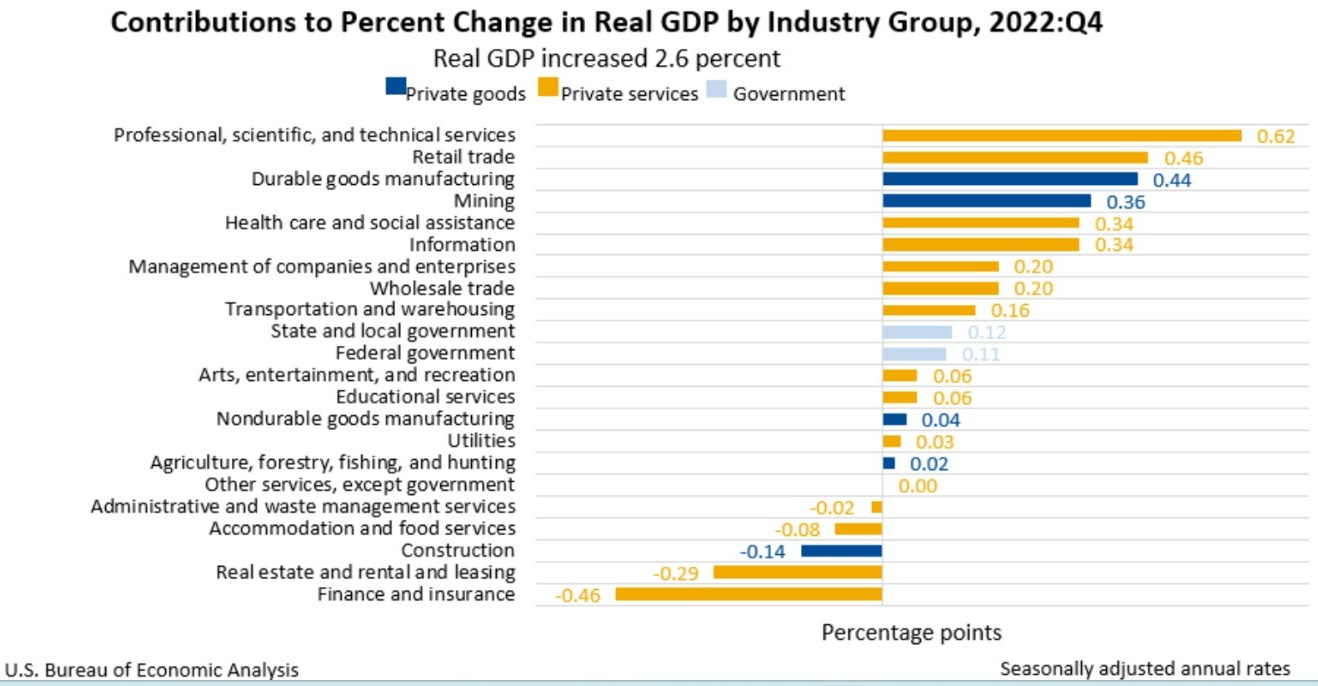
\includegraphics[width=10cm]{./style_files_stanford/industry.jpg}
 \end{figure}
\end{frame}

\begin{frame}[allowframebreaks]{Dupont Analysis}
		\begin{table}[!ht]
		%\small
		\fontsize{6.5}{20}\selectfont
		\centering
		\begin{tabular}{|c|c|c|c|c|c|c|c|c|c|c|c}
			\hline
			\rowcolor{blue}
			   &2017 & \makecell{2018} & \makecell{2019} & 2020&2021&\rowcolor{green}2022&2023&2024\\%&CR&P/S\\
			\hline
			Net Profit
			Margin&2.81\% &1.97\%&1.30\%&2.84\%&2.42\%&2.65\%&2.90\%&3.17\%\\%&25.42&0.710\\
			x Total Asset Turnover&2.44 &2.45 &2.35 &2.22 &2.21 &2.15 &2.08 &2.02 \\
			x (1 + D/E)&2.47 &2.53 &2.75 &2.90 &2.88 &3.01 &3.15 &3.29 \\
		= Return on Equity&16.94\%&12.20\%&8.38\%&18.25\%&15.43\%&17.14\%&19.04\%&21.14\%\\
			\hline
		\end{tabular}
	\end{table}

\end{frame}


\begin{frame}[allowframebreaks]{WACC, DDM, FCFF \& FCFE MODELS}
	\begin{itemize}
		\item The market price is \$139.81
	\end{itemize}
   \begin{table}[!ht]
	%\small
	\fontsize{15}{25}\selectfont
	\centering
	\begin{tabular}{|c|c|c|}
		\hline
		\rowcolor{blue}
	& \rowcolor{green}2022\\%&CR&P/S\\
		\hline
	WACC&  6.02\%\\%&25.42&0.710\\
		DDM  & \$130.61 \\
	FCFF&\$113.81 \\
	FCFE & \$131.68\\
		\hline
	\end{tabular}
   \end{table}
\end{frame}


\begin{frame}[allowframebreaks]{Conclusion}
\begin{itemize}
	\item Walmart has its sales growing and has maintained better net and gross margin than its peer competitors. 
	\item Any risk averse investor would like to hold Walmart Inc shares for a long time.
	\item As Walmart Inc stock is relatively safe, it is not a bad idea to hold already owned share for long term. \item Currently as the stock is overvalued, we recommend investors not to buy Walmart Inc stock right now. 
\end{itemize}

                
\end{frame}

%\begin{frame}[allowframebreaks]{Conclusion}
	
	
%\end{frame}



\end{document}